\section{Auswertung}
\subsection{Messung des Kontrasts}
Zur Bestimmung des Kontrastes des Interferometers wird ein Laser mit einer Wellenlänge von $\lambda = \SI{623,99}{\nano \meter}$ verwendet. Aus den in Tabelle \ref{tab:Kontrast} zu sehenden Werten wird der Kontrast
\begin{equation}
    K_\text{exp} = \frac{U_\text{Max}-U_\text{Min}}{U_\text{Max}+U_\text{Min}}
\end{equation}
berechnet.
\begin{table}[H] 
   \centering 
   \caption{Aufgenommene Messwerte zur Messung des Kontrastes.} 
   \label{tab:Kontrast} 
   \begin{tabular} { c c c c } 
 \toprule 
 {$Winkel\:/\: \mathrm{°}$} & {$U_\text{max}\:/\: \mathrm{mV}$} & {$U_\text{min}\:/\: \mathrm{mV}$} & {Kontrast}\\ 
    \midrule 
      0 & 1,12 & 0,90 & 0.1089108 \\ 
     15 & 2,10 & 0,73 & 0.4840989 \\ 
     30 & 2,90 & 0,33 & 0.7956656 \\ 
     45 & 3,45 & 0,15 & 0.9166666 \\ 
     60 & 2,94 & 0,25 & 0.8432601 \\ 
     75 & 1,98 & 0,69 & 0.4831460 \\ 
     90 & 1,16 & 0,98 & 0.0841121 \\ 
    105 & 1,25 & 0,39 & 0.5243902 \\ 
    120 & 1,02 & 0,08 & 0.8545454 \\ 
    135 & 0,89 & 0,03 & 0.9347826 \\ 
    150 & 0,82 & 0,20 & 0.6078431 \\ 
    165 & 0,88 & 0,38 & 0.3968254 \\ 
    180 & 1,03 & 0,86 & 0.0899470 \\ 
    \bottomrule 
  \end{tabular}
\end{table}


Die daraus erhaltenen Daten werden dann, wie in Abbildung \ref{fig:Kontrast} zu sehen ist, an die Funktion
\begin{equation}
    K = A \cdot | \sin{(2 \cdot \phi -\delta)} |
\end{equation}
\begin{center}
    \tiny{($A, \delta \hat{=} \text{Fitparameter} $)}
\end{center}
gefittet.
\begin{figure}[H]
    \centering
    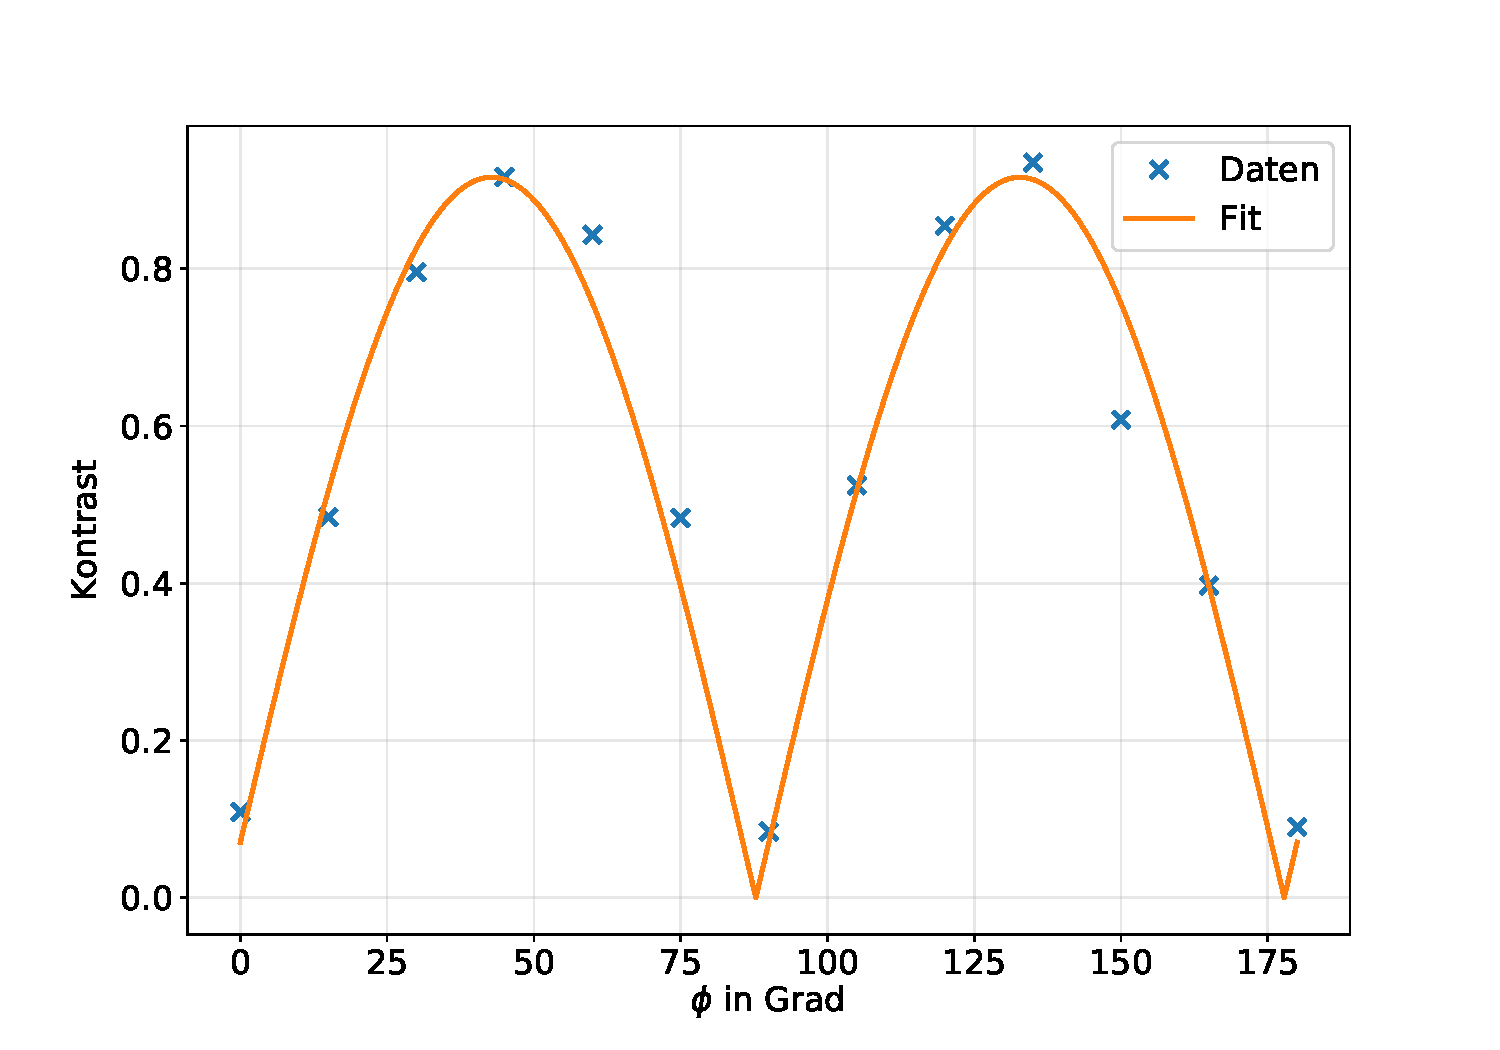
\includegraphics[width=0.8\textwidth]{data/kontrast.pdf}
    \caption{Messwerte für den winkelabhängigen Verlauf des Kontrastes.}
    \label{fig:Kontrast}
\end{figure}
Es ergeben sich die folgenden Fit-Parameter:
\begin{align}
       A &=  -0,077 \pm 0.026 \\
  \delta &=  0,916 \pm 0.025
\end{align}

\subsection{Bestimmung des Brechungsindex von Glas}
Die Bestimmung des Brechungsindex $n$ für Glas erfolgt mit dem in Gleichung \ref{eqn:brechungsindex_glas} aufgestellten Zusammenhang zwischen der Anzahl der Interferenzmaxima $M$ und $n$.
Bei einer Rotation um $\SI{11}{\degree}$ und einer Wandstärke $D = \SI{1}{\milli \meter} $ wurden die in Tabelle \ref{tab:M} zu sehenden Anzahl an Interferenzmaxima gemessen.
\begin{table}[H] 
    \centering 
    \caption{Gemessene Anzahl der Maxima M für Glas } 
    \label{tab:M} 
    \begin{tabular} { c } 
  \toprule 
  {Anzahl der Maxima M} \\ 
     \midrule 
     39 \\
     36 \\
     37 \\
     36 \\
     37 \\
     36 \\
     37 \\
     38 \\
     38 \\
     41 \\ 
     \bottomrule 
     {Durchnschittliche Maxima } \\
     \bottomrule 
      37,5
   \end{tabular}
 \end{table}

Damit folgt für den Brechungsindex von Glas
\begin{equation}
    n_\text{Glas} = 1,549 \pm 0,011 .
\end{equation}

\subsection{Bestimmung des Brechungsindex von Luft}
Mit der Gleichung \ref{eqn:brechungsindex_gas} und den in Tabellen \ref{tab:brechungsindex_gas1}, \ref{tab:brechungsindex_gas2} und \ref{tab:brechungsindex_gas3} zu sehenden Messwerten lässt sich der Brechungsindex von Luft für jede Messreihe berechnen. Dabei beträgt die Länge der Gaszelle $L = \SI{10}{\centi \meter}$.
\begin{table}[H] 
   \centering 
   \caption{Erste Messreihe zum Brechungsindex von Luft in 50 mbar Schritten. } 
   \label{tab:brechungsindex_gas1} 
   \begin{tabular} { c c c } 
 \toprule 
 {$Druck\:/\: \mathrm{mbar}$} & {$M1$} & {$n1$} \\ 
    \midrule 
     50  &  2 & 1,01266 \pm 0,00001 \\ 
     100 &  4 & 1,02532 \pm 0,00003 \\ 
     150 &  7 & 1,04431 \pm 0,00004 \\ 
     200 &  8 & 1,05064 \pm 0,00005 \\ 
     250 & 10 & 1,06330 \pm 0,00006 \\ 
     300 & 12 & 1,07596 \pm 0,00008 \\ 
     350 & 14 & 1,08862 \pm 0,00009 \\ 
     400 & 16 & 1,10128 \pm 0,00010 \\ 
     450 & 19 & 1,12027 \pm 0,00012 \\ 
     500 & 24 & 1,15192 \pm 0,00015 \\ 
     550 & 25 & 1,15825 \pm 0,00016 \\ 
     600 & 28 & 1,17724 \pm 0,00018 \\ 
     650 & 30 & 1,18990 \pm 0,00019 \\ 
     700 & 32 & 1,20256 \pm 0,00020 \\ 
     750 & 35 & 1,22155 \pm 0,00022 \\ 
     800 & 38 & 1,24054 \pm 0,00024 \\ 
     850 & 40 & 1,25320 \pm 0,00025 \\ 
     900 & 42 & 1,26586 \pm 0,00027 \\ 
     950 & 44 & 1,27852 \pm 0,00028 \\ 
    1000 & 46 & 1,29118 \pm 0,00029 \\ 
    \bottomrule 
  \end{tabular}
\end{table}
\begin{table}[H] 
   \centering 
   \caption{Zweite Messreihe zum Brechungsindex von Luft in 50 mbar Schritten.} 
   \label{tab:brechungsindex_gas2} 
   \begin{tabular} { c c c } 
 \toprule 
 {$Druck\:/\: \mathrm{mbar}$} & {$M2$} & {$n2$} \\ 
    \midrule 
      50 &  3 & 1.00001899 \pm 0.00000002 \\ 
     100 &  5 & 1.00003165 \pm 0.00000003 \\ 
     150 &  7 & 1.00004431 \pm 0.00000004 \\ 
     200 &  9 & 1.00005697 \pm 0.00000006 \\ 
     250 & 13 & 1.00008229 \pm 0.00000008 \\ 
     300 & 15 & 1.00009495 \pm 0.00000009 \\ 
     350 & 17 & 1.00010761 \pm 0.00000011 \\ 
     400 & 19 & 1.00012027 \pm 0.00000012 \\ 
     450 & 21 & 1.00013293 \pm 0.00000013 \\ 
     500 & 23 & 1.00014559 \pm 0.00000015 \\ 
     550 & 26 & 1.00016458 \pm 0.00000016 \\ 
     600 & 27 & 1.00017091 \pm 0.00000017 \\ 
     650 & 31 & 1.00019623 \pm 0.00000020 \\ 
     700 & 34 & 1.00021522 \pm 0.00000022 \\ 
     750 & 37 & 1.00023421 \pm 0.00000023 \\ 
     800 & 38 & 1.00024054 \pm 0.00000024 \\ 
     850 & 40 & 1.00025320 \pm 0.00000025 \\ 
     900 & 42 & 1.00026586 \pm 0.00000027 \\ 
     950 & 44 & 1.00027852 \pm 0.00000028 \\ 
    1000 & 47 & 1.00029751 \pm 0.00000030 \\ 
    \bottomrule 
  \end{tabular}
\end{table}


\begin{table}[H] 
   \centering 
   \caption{Dritte Messreihe zum Brechungsindex von Luft in 50 mbar Schritten.} 
   \label{tab:brechungsindex_gas3} 
   \begin{tabular} { c c c } 
 \toprule 
 {$Druck\:/\: \mathrm{mbar}$} & {$M3$} & {$n3$} \\ 
    \midrule 
      50 &  2 & 1,01266 \pm 0,00001 \\ 
     100 &  4 & 1,02532 \pm 0,00003 \\ 
     150 &  6 & 1,03798 \pm 0,00004 \\ 
     200 & 12 & 1,07596 \pm 0,00008 \\ 
     250 & 17 & 1,10761 \pm 0,00011 \\ 
     300 & 19 & 1,12027 \pm 0,00012 \\ 
     350 & 21 & 1,13293 \pm 0,00013 \\ 
     400 & 23 & 1,14559 \pm 0,00015 \\ 
     450 & 28 & 1,17724 \pm 0,00018 \\ 
     500 & 28 & 1,17724 \pm 0,00018 \\ 
     550 & 29 & 1,18357 \pm 0,00018 \\ 
     600 & 32 & 1,20256 \pm 0,00020 \\ 
     650 & 34 & 1,21522 \pm 0,00022 \\ 
     700 & 36 & 1,22788 \pm 0,00023 \\ 
     750 & 36 & 1,22788 \pm 0,00023 \\ 
     800 & 41 & 1,25953 \pm 0,00026 \\ 
     850 & 43 & 1,27219 \pm 0,00027 \\ 
     900 & 47 & 1,29751 \pm 0,00030 \\ 
     950 & 51 & 1,32282 \pm 0,00032 \\ 
    1000 & 54 & 1,34181 \pm 0,00034 \\ 
    \bottomrule 
  \end{tabular}
\end{table}
Mithilfe dieser Werte kann anschließend, wie in Abbildung \ref{fig:n} zu sehen,  eine lineare Regression der Form 
\begin{equation}
    f(x, a, b) = a \cdot \frac{x}{T \cdot R} + b
    \label{eqn:fit}
\end{equation}
durchgeführt werden. Dabei gehen die Temperatur $T = \SI{20,5}{\celsius} $ und die universelle Gaskonstante $R$ als Konstanten in den Fit ein. 
\begin{figure}[H]
    \centering
    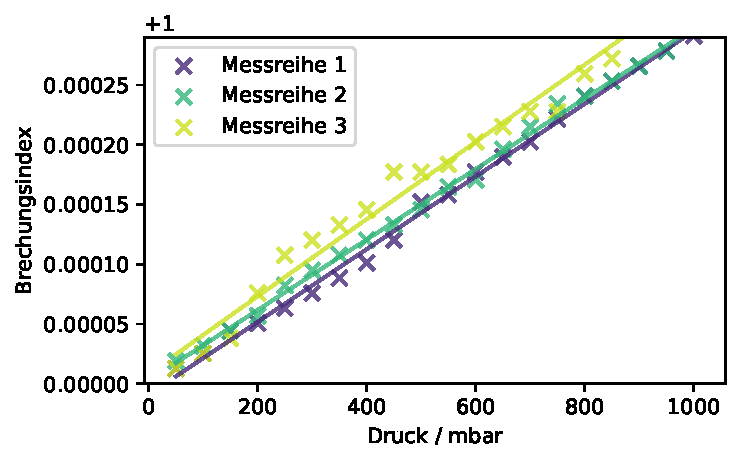
\includegraphics[width=0.8\textwidth]{data/Plots/Brechungsindex.pdf}
    \caption{Brechungsindices aufgetragen gegen den Druck. }
    \label{fig:n}
\end{figure}
Es ergeben sich die in Tabelle \ref{tab:fit} zu sehenden Fitparameter.
\begin{table} 
    \centering 
    \caption{Ermittelte Regressionsparameter $A$ und $B$ der Messung zur Bestimmung der Abhängigkeit zwischen Brechungsindex $n$ und Druck p. Zudem ist jeweils der Wert $n_{\mathup{norm}}$ zum Vergleich mit der Literatur angegeben.} 
    \label{tab:fit} 
    \begin{tabular}{c c c}
    \toprule  
    {Messung} & {$a \:/\: \si{ 10^{-7}\milli\bar}$} & {$b$} \\ 
    \midrule  
    1 & 3,042160712 \pm 0,04510441 & 0.99999093 \pm 0,0000027 \\ 
    2 & 2,950785567 \pm 0,03474827 & 1.00000269 \pm 0,0000020 \\ 
    3 & 3,231580017 \pm 0,10051475 & 1.00000852 \pm 0,0000060 \\ 
    \bottomrule 
    \end{tabular} 
    \end{table}
    
Damit ergeben sich mithilfe des Lorentz-Lorenz Gesetz bei einem Druck von $p = \SI{1013}{\milli \bar}$ folgende Brechungsindices:
\begin{align}                                 
    n(p = \SI{1013}{\milli \bar}, \SI{20,5}{\celsius} )_\text{Luft, 1} = 1.00029910 \pm 0,00000530   \\
    n(p = \SI{1013}{\milli \bar}, \SI{20,5}{\celsius} )_\text{Luft, 2} = 1.00030161 \pm 0,00000408   \\
    n(p = \SI{1013}{\milli \bar}, \SI{20,5}{\celsius} )_\text{Luft, 3} = 1.00033588 \pm 0,00001182  
\end{align}
Eine Mittelung über alle Werte ergibt folglich:
\begin{equation}
    n(p = \SI{1013}{\milli \bar}, \SI{20,5}{\celsius} )_\text{Luft} = 1.000312 \pm 0.000005
\end{equation}
Mithilfe von Gleichung \eqref{eqn:fit} werden daraufhin die Brechungsindices für $T = \SI{15}{\celsius}$
berechnet:
\begin{align}                                 
    n(p = \SI{1013}{\milli \bar}, \SI{15}{\celsius} )_\text{Luft, 1} = 1,00030555 \pm 0,00000539 \\
    n(p = \SI{1013}{\milli \bar}, \SI{15}{\celsius} )_\text{Luft, 2} = 1.00030786 \pm 0,00000415 \\
    n(p = \SI{1013}{\milli \bar}, \SI{15}{\celsius} )_\text{Luft, 3} = 1.00034273 \pm 0,00001201
\end{align}
Eine Mittelung über diese Werte ergibt:
\begin{equation}
    n(p = \SI{1013}{\milli \bar}, \SI{15}{\celsius} )_\text{Luft} = 1.000319 \pm 0.000005
\end{equation}